\documentclass[crop,border=0pt]{standalone}

\usepackage{mathtools}
\usepackage{tikz}
\usetikzlibrary{positioning,decorations.pathreplacing,scopes,arrows}

\begin{document}
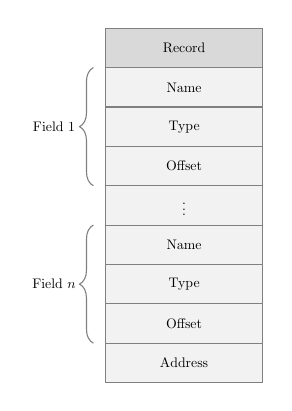
\begin{tikzpicture}[scale=0.5, every node/.style={scale=0.5,black}]
  {[xstep=4cm, ystep=1cm, gray, thin]

    \draw[fill=gray!10] (0, 0) grid (4, 8) rectangle (0, 0);
    \draw[fill=gray!30] (0, 8) grid (4, 9) rectangle (0, 8);

    \node at (2, 8.5) {Record};
    \node at (2, 7.5) {Name};
    \node at (2, 6.5) {Type};
    \node at (2, 5.5) {Offset};
    \node at (2, 4.5) {\(\vdots\)};
    \node at (2, 3.5) {Name};
    \node at (2, 2.5) {Type};
    \node at (2, 1.5) {Offset};
    \node at (2, 0.5) {Address};

    \draw
    [decorate,decoration={brace,amplitude=5pt},xshift=-0.1,yshift=0pt]
    (-0.3,5) -- (-0.3,8) node [black,midway,xshift=-1cm] {Field 1};

    \draw
    [decorate,decoration={brace,amplitude=5pt},xshift=-0.1,yshift=0pt]
    (-0.3,1) -- (-0.3,4) node [black,midway,xshift=-1cm] {Field \(n\)};
  }

\end{tikzpicture}
\end{document}
